
\ChapterWithSubtitle{IR Absorption by GH Gases (F25: 2 Weeks)}{I am back to save the universe}
%\chapter{Heating by Radiation}

%%%%%%%%%%%%%%%%%%%%%%%%%%%%%%%%%%%%%%%%%%%%%
\section*{Equipment List}

\begin{multicols}{2}   % change 2 -> 3 for three columns
\begin{equipment}
\item Ruler
\item Digital Thermometer
\item Sharpie
\item 250 mL beaker 
\item 500 mL beaker 
\item Hot Plate
\item Lab jack
\item IR thermal imaging camera
\item IR thermometer
\item plastic basket with windows
\item Voltage amplifier box and wires
\item Cardboard box ``tunnel'' for restricting thermopile's field of view
\item Digital multimeter (DMM)
\item Various narrow-band thermopiles (\unit{3.375}{\micro\meter}, \unit{3.91}{\micro\meter}, \unit{4.3}{\micro\meter}, \unit{4.43}{\micro\meter}) and a broad-spectrum thermopile (\unit{8}{\micro\meter} -- \unit{14}{\micro\meter})
\item ziploc-style  bags (for classroom)
\end{equipment}
\end{multicols}


%%%%%%%%%%%%%%%%%%%%%%%%%%%%%%%%%%%%%%%%%%%%%
\section{Introduction and Definitions}

\subsection{Climate Sensitivity}

This week in class we are attempting to identify the precise connection between additional greenhouse gases in the atmosphere and the resulting temperature increase.  This connection is called the {\bf climate sensitivity}\footnote{{\em Climate sensitivity} is often used as a technical term by climate scientists to refer to ``the temperature increase due to a doubling of atmospheric $\text{CO}_2$''; but it is also used in this more general sense.}.  In lecture and discussion, we will attempt to see this connection through the deepening and broadening of $\text{CO}_2$ absorption lines in the blackbody spectrum of the Earth surface's infrared radiation. Here, in lab, we will simply try to quantitatively observe the absorption of infrared light by $\text{CO}_2$ (and possilbly air and water vapor).

\subsection{Absorption lines and IR thermometer/camera measurements}

Previously in Discussion we learned how to draw blackbody spectra on log-log paper and then, when studying the IR absorption by greenhouse gases, we sketched absorption lines on these spectra.  Recall the relevant equations for this process:
	%
	\begin{equation*}
	\lambda_\text{peak} = \frac{\unit{2900}{\micro\meter \cdot \kelvin}}{T}  \quad ; \quad
	F = \left( 5.7 \times 10^{-8} \, \frac{\text{J}/\text{s}}{\text{m}^2 \cdot \text{K}^4}\right) T^4 \quad ; \quad
	F_\lambda = \frac{F}{1.5 \times \lambda_\text{peak}}
	\end{equation*}
	%
To create the blackbody curve, we drew the peak (``hat'') with three points at wavelengths of $[ \frac{\lambda_p}{2}, \lambda_p, 3 \lambda_p]$, and at spectral flux values of $[\frac{F_\lambda}{10}, F_\lambda, \frac{F_\lambda}{10} ]$; the curve dropped off with a slope of 4 to high wavelengths, and more quickly at low wavelengths.\\[6pt]

\noindent On a single piece of log-log graph paper, draw blackbody curves for the following temperatures: room temperature ($20\degree\text{C} = \unit{293}{\kelvin}$); hot water ($50\degree\text{C} = \unit{323}{\kelvin}$); boiling water ($100\degree\text{C} = \unit{373}{\kelvin}$); and a heat lamp at $450\degree\text{C} = \unit{673}{\kelvin}$. Make your calculations here:


\answerspace[7cm]

\noindent We will attempt to see the absorption of infrared light by carbon dioxide using IR thermometer guns and imaging cameras, but this is not a completely straightforward process because of how these devices work.  First, they estimate temperature by collecting all light over a range of wavelengths, 8--\unit{14}{\micro\meter}.  They measure the total flux emitted by an object in that wavelength range and then compare it to what would be expected from blackbody curves at different temperatures (the ``area under the curve'' between these wavelengths).  On your blackbody graph, draw two vertical lines to indicate this range of wavelengths.  Looking at your curves, which of the objects would have the most flux in this range.  Can you estimate how much more\footnote{An approximation to the observed total flux is the area of a rectangle that has height $F_\lambda$ (at the center of the 8--\unit{14}{\micro\meter} interval) and width: $\unit{14}{\micro\meter} - \unit{8}{\micro\meter} = \unit{6}{\micro\meter}$.} it is than the second most?

\answerspace

\noindent A second issue with these devices is that their wavelength range has been specifically chosen to {\em avoid} the $\text{CO}_2$ absorption lines, which (remember from our {\em Infrared Absorption} discussion) are at \unit{4.3}{ \micro\meter} and \unit{15}{\micro\meter}.  Draw vertical lines on your blackbody curve to indicate these wavelengths.  Is it possible that a carbon dioxide absorption line will affect anything in the 8--\unit{14}{\micro\meter} sensitivity range of the devices?  Why or why not?

\answerspace

\noindent We do expect to see some small effect because of the line width of carbon dioxide, particularly at \unit{15}{\micro\meter}.  As that line takes a bite out of the spectrum, it should cover a small part of the sensitivity range of the devices.  Sketch absorption ``valleys'' on each of your spectra at both the \unit{4.3}{\micro\meter} and  \unit{15}{\micro\meter} locations.  Looking at your graphs, do you expect that any of the three non-room-temperature sources would be more affected\footnote{I don't think there is a clear-cut answer to this, particularly from our approximate blackbody curves, but it is an interesting question to think about.} than others?



\newpage
%%%%%%%%%%%%%%%%%%%%%%%%%%%%%%%%%%%%%%%%%%%%%
%%%%%%%%%%%%%%%%%%%%%%%%%%%%%%%%%%%%%%%%%%%%%


%%%%%%%%%%%%%%%%%%%%%%%%%%%%%%%%%%%%%%%%%%%%%
\section{Experiments and Analysis}

{\bf \underline{Safety Notes}:} 
	%
	\begin{itemize}
	\item We have tanks of $\text{CO}_2$ and $\text{N}_2$ gas in the classroom.  Do not disturb their buckle attachments to the table as the greatest danger would be for them to fall, break a valve and then ``rocket'' across the room.  Be gentle when screwing the valves to release the gases.
	\item We will use a hot plate as a thermal radiation source. It is hanging vertically, so be careful not to touch or brush up against it.
	\end{itemize}
	
\noindent As always: \underline{read the full procedures} prior to beginning any experimentation.

\subsection{IR transparency of plastic bags}

Make some measurements and observations to test  transparency of the plastic bags we will later fill with gas.  There are multiple types of bags that can be used (multiple ``Ziploc''-style, and food-storage ``produce'' bags). You can use IR thermometer gun and the IR imaging camera.  Observe what is visible in the camera image and how the measurements of temperature recorded by both devices changes through one or multiple plastic bag layers.  You can use humans as sources of IR or fill a beaker with ``hot'' tap water.\\[-6pt]

\noindent Record your observations, measurements, and conclusions here.

\answerspace[7cm]


\subsection{IR absorption in air}

Complete the steps below with your table of four using the Mileseey infrared camera. We are interested in the device's measured temperature of the vat of water at different distances, but because it is cooling in the room over time, we need to observe that cooling for a few minutes at each distance and then extrapolate backwards to obtain an estimate of the initial temperature for each distance. \\


%%%%%%%%%%%%%%%%%%%%%
\newpage

\noindent {\bf Procedure:} 
	%
	\begin{itemize}
	\item Starting at the vat of hot water (tap water at $\sim 50\degree$C), use a meter stick (located along the walls on top of the power strip) to mark out  distances of \unit{1}{\meter}, \unit{2}{\meter}, \unit{3}{\meter}, \unit{4}{\meter}, and \unit{5}{\meter} with masking tape on the floor.
	\item Start your stopwatch.
	\item Use the IR camera to make measurements of the temperature of the vat of water from zero to five meters, recording the time, distance, and temperature. You should be able to use the (red) ``max'' temperature value shown on the image (or the white central cross-hairs temperature shown at top left).  These measurements will probably be 20--30 seconds apart. Enter these values in a three-column table in Google Sheets, recording the time in two columns, minutes and seconds, so that you can later convert to ``t (s)''.
	\item Repeat the zero to five meter measurements 5--7 times.
	\end{itemize}
	%

\noindent {\bf Analysis:} Copy the Google Sheets table for each student. Using the two time columns, create a ``time in seconds'' column (with an excel command like ``\verb|=A2*60+B2|'').  On a single sheet of graph paper, plot six data sets for the Temperature vs.\ time values at each distance (make each axis range as narrow as possible while still showing the data \ldots it is not necessary to show the ``origin'').  [Alternatively you could copy your data into separate sheets for each distance and insert Charts for each.]  Using a ruler, draw a line of best fit and obtain the ``y intercept,'' i.e., the temperature at time zero, for each of the datasets.  Then make a new plot, on another sheet of graph paper, showing initial temperature vs.\ distance.\\[-6pt]

\noindent Briefly state what you observe in each of the two graphs.  How do your results demonstrate absorption of IR light, if at all?  If there is IR absorption, what do you think is the primary contributor?

\answerspace

\vfill

--- End of Day 1 ---

%%%%%%%%%%%%%%%%%%%%%
\newpage


\subsection{IR absorption by $\text{CO}_2$ (effect on reported temperature)}

We will use a hot plate for our infrared radiation source and observe the reported temperature by an IR thermometer gun through bags of gas. You can set the hot plate to the max temperature value or, following your analysis in the introduction of blackbody curves and absorption lines, choose a different temperature of the source.  You will observe this source through three bags of gas: first all three nitrogen; then replacing each nitrogen, one-by-one, with carbon dioxide.  Then you will repeat this process using bags of air. You will measure the temperature of the source through the bags in each case and seek some effect of carbon dioxide absorption.  \\[-6pt]

\noindent {\bf Procedure:}
	%
	\begin{itemize}
	\item Set up your hot plate vertically,  turn it on, and set its temperature.
	\item Using the tanks of $\text{CO}_2$ and $\text{N}_2$ gas, fill three clear quart-size, ziploc-style bags of each gas (avoid bags if the lettering/logo blocks the line-of-sight). Label each at the bottom of the bag using a Sharpie, indicating its contents.  When using the tanks: the main tank valve should be {\em unscrewed} (CCW) a little bit from the closed position.  Then the secondary valve (thin bar) is {\em screwed in} (CW) to make the gas come out. Your instructor will help you with this. Be gentle with the screwing and unscrewing, and try not to let too much gas escape when filling. Fill the bags up as full as you can. When finished, close the tank valves again.
	\item Fill three more bags with air from the room, using the small orange pumps. [Alternatively, you could use your breath to fill these bags, which will contain a higher concentration of $\text{CO}_2$ than air ($\sim 3\%$ rather than $0.0425\%=\unit{425}{ppm}$), and possibly some water vapor.]
	\item Place your windowed basket on the lab jack and point it toward the hot plate source.  Place blue masking tape on the table to record the distance of your basket from the hot plate; measure that distance and record it.  To avoid burning the bags/basket, this should not be too close, probably around \unit{40}{\centi\meter}.  Once your hot plate has reached a constant temperature as measured by your thermometer gun, record both the hot plate temperature setting and the actual temperature.
	\item Create a table, on paper or Google Sheets, to record temperature measurements.  You should have four columns: [$N_{\text{CO}_2}$, $N_{\text{N}_2}$, $N_\text{air}$, $T$], to express the combination of bags.
	\item First record the temperature of the hot plate through the window of your empty basket. Be sure hold the trigger down, and scan the hot plate slowly to find the hottest point.  You will always record this maximum temperature.
	\item Then, start with three bags of nitrogen.  Make sure the bags are puffed up fully, e.g., by holding your hand flat across their tops if the bags are not completely full on their own. Also make sure the line of sight through the basket windows is pointed at the hot plate and there are no obstructions (e.g., folds/seams in the ziploc bags or  Record the temperature through the bags in your table.
	\item Replace one nitrogen bag with a carbon dioxide bag.  Again record the temperature.  Then replace another $\text{N}_2$ bag with $\text{CO}_2$ and repeat. Record your measurements in a table with columns noting the number of $\text{N}_2$ and $\text{CO}_2$ bags ($N_\text{air}$ will be zero for all of these measurements).
	\item Return to three nitrogen bags and then replace them sequentially with the air bags.
	\item Turn off your hot plate.
	\end{itemize}
	

\noindent {\bf Analysis:}   Make two graphs:  temperature vs carbon dioxide bag number, and temperature vs.\ air bag number. In the space below, describe what you have seen and decide if you have observed any absorption by carbon dioxide (or in the case of the air bag, absorption by either carbon dioxide or water vapor).

\answerspace[8cm]

\noindent Why did we use nitrogen as the comparison gas?

\answerspace


%\subsection{IR absorption by wet $\text{CO}_2$ (OPTIONAL)}
%Repeat the prior experiment, but filling the bags with carbon dioxide generated with baking soda and vinegar.

\subsection{IR absorption by $\text{CO}_2$  (an absorption spectrum)}

With your table of four, you will now attempt to see the wavelength dependence of infrared absorption by $\text{CO}_2$. We will again use the hot plate as the IR source, this time at maximum temperature.  We have a collection of four narrow-band infrared {\em thermopiles} (the same detector that is used within the thermometer guns, but restricted to a very narrow wavelength band around their central value, rather than $8$--\unit{14}{\micro\meter}), as well as a broad-band thermopile for comparison. These thermopiles output a miniscule voltage (in the hundreds of microvolts range) which we can amplify into hundreds of millivolts and observe with the digital multimeter (DMM).  We will again compare observations through bags of nitrogen, carbon dioxide, and air; but this time using only a single bag held in front of the thermopile. \\[-6pt]

%%%%%%%%%%%%%%%%%%%%%
\newpage

\noindent{\bf Equipment Notes}:
	%
	\begin{itemize}
	\item The DMM should be set to voltage (the ``$\text{V}\sim$'' selection) on the dial, and then switched to ``DC'' voltage (from the ``AC'' default) by pressing ``Select'' button.  If the DMM powers off while using, press the Select button once to turn back on, and again to switch to DC voltage.
	\item The wire leads from the DMM will be directly connected to the various thermopile squares (red to red, black to black). Readings on the DMM from these devices will be small and often negative. This is ok, since only differences in voltage have physical meaning. High voltage values (e.g., less negative values) will correspond to higher infrared intensity. Be sure to include the sign of your voltage reading when recording data.  
	\item The connections of the DMM and the power source should be set up for you already, but ask your instructor if you have trouble getting readings, or think it might have been disconnected.
	\end{itemize}

\noindent{\bf Procedure}:
	%
	\begin{itemize}
	\item Set up using the hot plate that is facing away from the nearest wall so that you will point your thermopiles away from the center of the room (they are very sensitive to stray infrared light sources, like people). Turn on the hot plate and set to maximum temperature.
	\item Select nice plump bags of nitrogen, $\text{CO}_2$, and air, one bag for each gas.
	\item Create a Google sheet, with columns for: 
		%
		\begin{quote}
		[$\lambda$, Vhp (no bag), Vhp (N2), Vhp (CO2), Vhp (air), Vw (no bag)]%, Vw (N2)]
		\end{quote}
	where ``V'' stands for voltage, ``hp'' stands for hot plate (measurements pointed at the hot plate), and ``w'' stands for wall (baseline measurements pointed at the wall, at approximately room temperature). There will be five rows --- one for each narrow-band thermopile, and one broadband (8--\unit{14}{\micro\meter}) --- with wavelength $\lambda$ values \{3.375, 3.91, 4.3, \unit{4.43}{\micro\meter}\}.
	\item Set the cardboard box tunnel on the top of the lab jack and raise it such that the box is pointed at the center of the hot plate.  Attach binder clips to the sides of the back of the lab jack platform and push the ends of the red and black wire leads through the binder clips (so the wires are ready to be plugged into a thermopile).  
	\item This time, the lab jack can be about \unit{20}{\centi\meter} away from the hotplate when making measurements (since we will not leave bags near the hot plate). Set its distance, measure it, and place tape on the table so that it can be easily positioned.  Before measurements it can be moved away to avoid getting too hot.
	\item Once the hot plate has reached a steady temperature, record its stated value and the actual value measured with the infrared thermometer gun.
	\item Select one of the five thermopiles from the thermopile library provided to the class as a whole. Attach the red and black wires to it and push it into the ``back window'' of the cardboard box (the one that goes to the bottom).
	\item Recording voltage measurements: (i) prop the DMM on its stand so that it can easily be read; (ii) have one person stand very still to the side of the table, ready to hold bags between the box window and the hot plate; (iii) try to keep everyone else out of the field of view of the sensor (or the ``reflection'' off the hot plate \ldots check out your own reflection in the aluminum baking sheet, using the thermal imaging camera!).
	\item Wait for the voltage reading to stabliize and record the ``Vhp (no bag)'' measurement.  Then hold the nitrogen bag in front of the ``front'' window of the cardboard box, wait for the voltage reading to stabilize, and record it.  Repeat for all other columns.  For the ``wall'' columns, move the lab jack away from the hot plate and point your sensor at the room-temperature wall.
	\item Switch to a different thermopile sensor and collect its data in the next row of your Sheet.
	\end{itemize}


\noindent {\bf Analysis:}   Because each sensor has a slightly different wavelength width and base voltage value, we will make a ``spectrum'' (for the carbon dioxide and air bags) by normalizing their values to the nitrogen values.  Make three new columns in your Google Sheet for the ``normalized voltages'', titled [VnN2, VnA, VnCO2]. The equation to get each of these values will be:
	%
	\begin{equation*}
	V_{\text{norm}, \text{gas}} = \frac{ V_{\text{hp}, \text{gas}} - V_{\text{wall (no bag)}} }{ V_{\text{hp}, \text{N}_2} - V_{\text{wall (no bag)}} }
	\quad \quad \left( \text{with ``gas'' } = \text{ N}_2, \text{CO}_2, \text{air}\right)
	\end{equation*}
	%
Explain what this equation means, in your own words.  What will be the value for each of the $\text{N}_2$ normalized voltages?

\answerspace

\noindent You can implement this equation using an Excel-style formula in your Google Sheet.  If the data for one thermopile is in row 2, with $\lambda$ in column A (and the voltage values listed above in the next columns), then a formula like this should work for the normalized $\text{CO}_2$ value:
	%
	\begin{quote}
	\verb| = (D2 - F2) / (C2 - F2) |
	\end{quote}
	%
Explain why this (or something close to it for your Sheet) matches the above equation for normalized voltage and the columns listed within the Procedure.

\answerspace


\noindent Type in the Excel formula for the first row in each of the normalized voltage columns; then drag the bottom right corner of the cell down to fill the values for all other thermopile rows. What do you see for the normalized voltages in the ``broadband'' (8--\unit{14}{\micro\meter}) thermopile?  Since this is the sensor in the IR thermometer guns, does this data support your findings from the prior experiments?  Why or why not?

\answerspace

\noindent Plot the normalized voltages vs.\ wavelength for $\text{N}_2$, $\text{CO}_2$, and air together on one (scatter) Chart (using only the narrow-band thermopiles, not the broadband). To make a Chart that displays multiple data sets, copy your single table into multiple copies in the manner shown in the figure below (Source: \href{https://www.reddit.com/r/googlesheets/comments/17sm8q5/comment/k8qyb0j/}{Reddit user 7FOOT7}). Notice that you should have three different rows with the same wavelength, one for each column of normalized voltages.  Highlight that full dataset, including its column labels (so it would be \verb|A1| to \verb|D10| in the example below), and do {\em Insert}/{\em Chart}.
%
\begin{center}
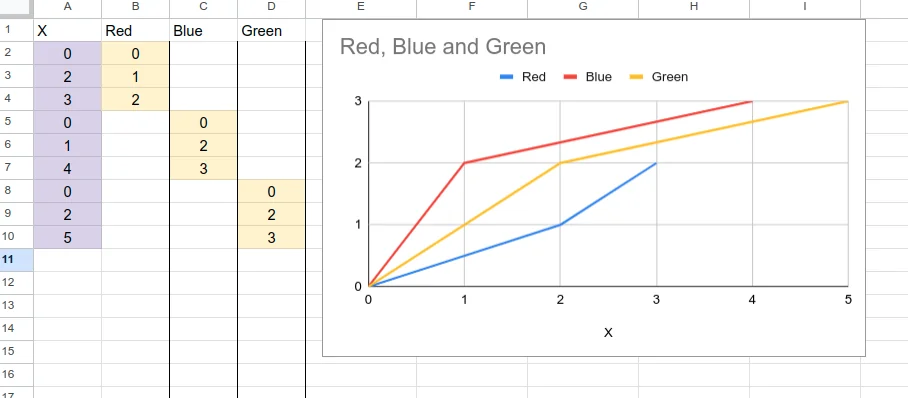
\includegraphics[width=\textwidth]{images/09_multiple-lines-on-chart-google-sheets.png}
\end{center}
%
What do you see in your spectrum?  Is there evidence of absorption by $\text{CO}_2$? How does the ``air'' spectrum compare to the $\text{CO}_2$ spectrum?  Try to give an explanation for the results in terms of what we have learned about greenhouse gases in other parts of the course.

\answerspace[5.5cm]

\noindent If you examine your data, comparing the ``Vhp (N2)''  and ``Vhp (CO2)'' raw values to the ``Vhp (no bag)'' values, you should see that there is one wavelength for which: (i) nitrogen and carbon dioxide have similar values, but (ii) both nitrogen and carbon dioxide are lower than at other wavelengths.  [If you would like, you can create another graph to see this clearly, by creating a normalized spectrum (now for $\text{CO}_2$, air, and $\text{N}_2$) to the ``Vhp (no bag)'' rather than to nitrogen.]  Do you see this? What is the explanation?





%{\em [F2025] We have an array of five narrow-band infrared sensors (thermopiles) from which one can measure input radiation as a voltage.  By comparing the radiation incident on the sensors through bags of nitrogen to that through bags of carbon dioxide, we can obtain an approximate spectrum showing the absorption line around \unit{4.3}{\micro\meter}.  Unfortunately we do not have the technical details of this experiment ready yet.  We will potentially revisit in a future week.}
	

\answerspace[7cm]



 